\documentclass{beamer}
\usetheme{Copenhagen}
%\usetheme{Boadilla}
\usepackage{geometry}                % See geometry.pdf to learn the layout options. There are lots.
\usepackage{graphicx}
\usepackage{amssymb}
 \usepackage{feynmp}
 \usepackage{textpos}
 \usepackage{biblatex}
 \usepackage{bbold}
  \usepackage{ulem}
  
\usepackage{color}
 \bibliography{foo}
  \DeclareGraphicsRule{*}{mps}{*}{} 
  % figures
  
 % \logo{
\includegraphics[height=1.2cm]{lhcblogo.jpg}\vspace{220pt}}
  
  
\usepackage{caption}
\usepackage{subfig}
\newcommand{\Lagr}{\mathcal{L}}
\setbeamertemplate{itemize item}{\scriptsize\raise1.25pt\hbox{\donotcoloroutermaths$\blacktriangleright$}}
\setbeamertemplate{itemize subitem}{\tiny\raise1.5pt\hbox{\donotcoloroutermaths$\square$}}
\setbeamertemplate{itemize subsubitem}{\tiny\raise1.5pt\hbox{\donotcoloroutermaths$\blacktriangleright$}}
\setbeamertemplate{enumerate item}{\insertenumlabel.}
\setbeamertemplate{enumerate subitem}{\insertenumlabel.\insertsubenumlabel}
\setbeamertemplate{enumerate subsubitem}{\insertenumlabel.\insertsubenumlabel.\insertsubsubenumlabel}
\setbeamertemplate{enumerate mini template}{\insertenumlabel}
\begin{document}

{


\title[  $\Lambda_{b} \rightarrow p \mu \nu$ Update \hspace{2em}\insertframenumber/
\inserttotalframenumber]{$\Lambda_{b} \rightarrow p \mu \nu$ Update }
\author[William Sutcliffe]{
\includegraphics[height=1cm,width=1.5cm]{lhcblogo.jpg} \\ William Sutcliffe}

\date{\today}

 \frame{\titlepage

} 

\addtobeamertemplate{frametitle}{}{%
\begin{textblock*}{100mm}(.85\textwidth,-1cm)

\includegraphics[height=1cm,width=1.5cm]{lhcblogo.jpg}
\end{textblock*}}

 %%%%slide 1

% \frame{\frametitle{Outline} 
%\begin{enumerate}
%\setlength{\itemsep}{10pt}
%\item Background and motivation.
%\item Previous measurements.
%\item $V_{ub}$ with LHCb
%\item Initial generator level study
%\end{enumerate}
%}






 \frame{
 \frametitle{Current Status of $|V_{ub}|$}
 \begin{itemize}
  \item \normalsize{Semi-Leptonic B Decays:}
   \end{itemize}
   \hspace{1.cm} \footnotesize{Inclusive ($\bar{B} \rightarrow X_{u} l \bar{\nu}_{l}$)} \hspace{1cm}  \footnotesize{Exclusive ($\bar{B}_{0} \rightarrow \pi^{+} l \bar{\nu}_{l}$)}
    \begin{center} 
    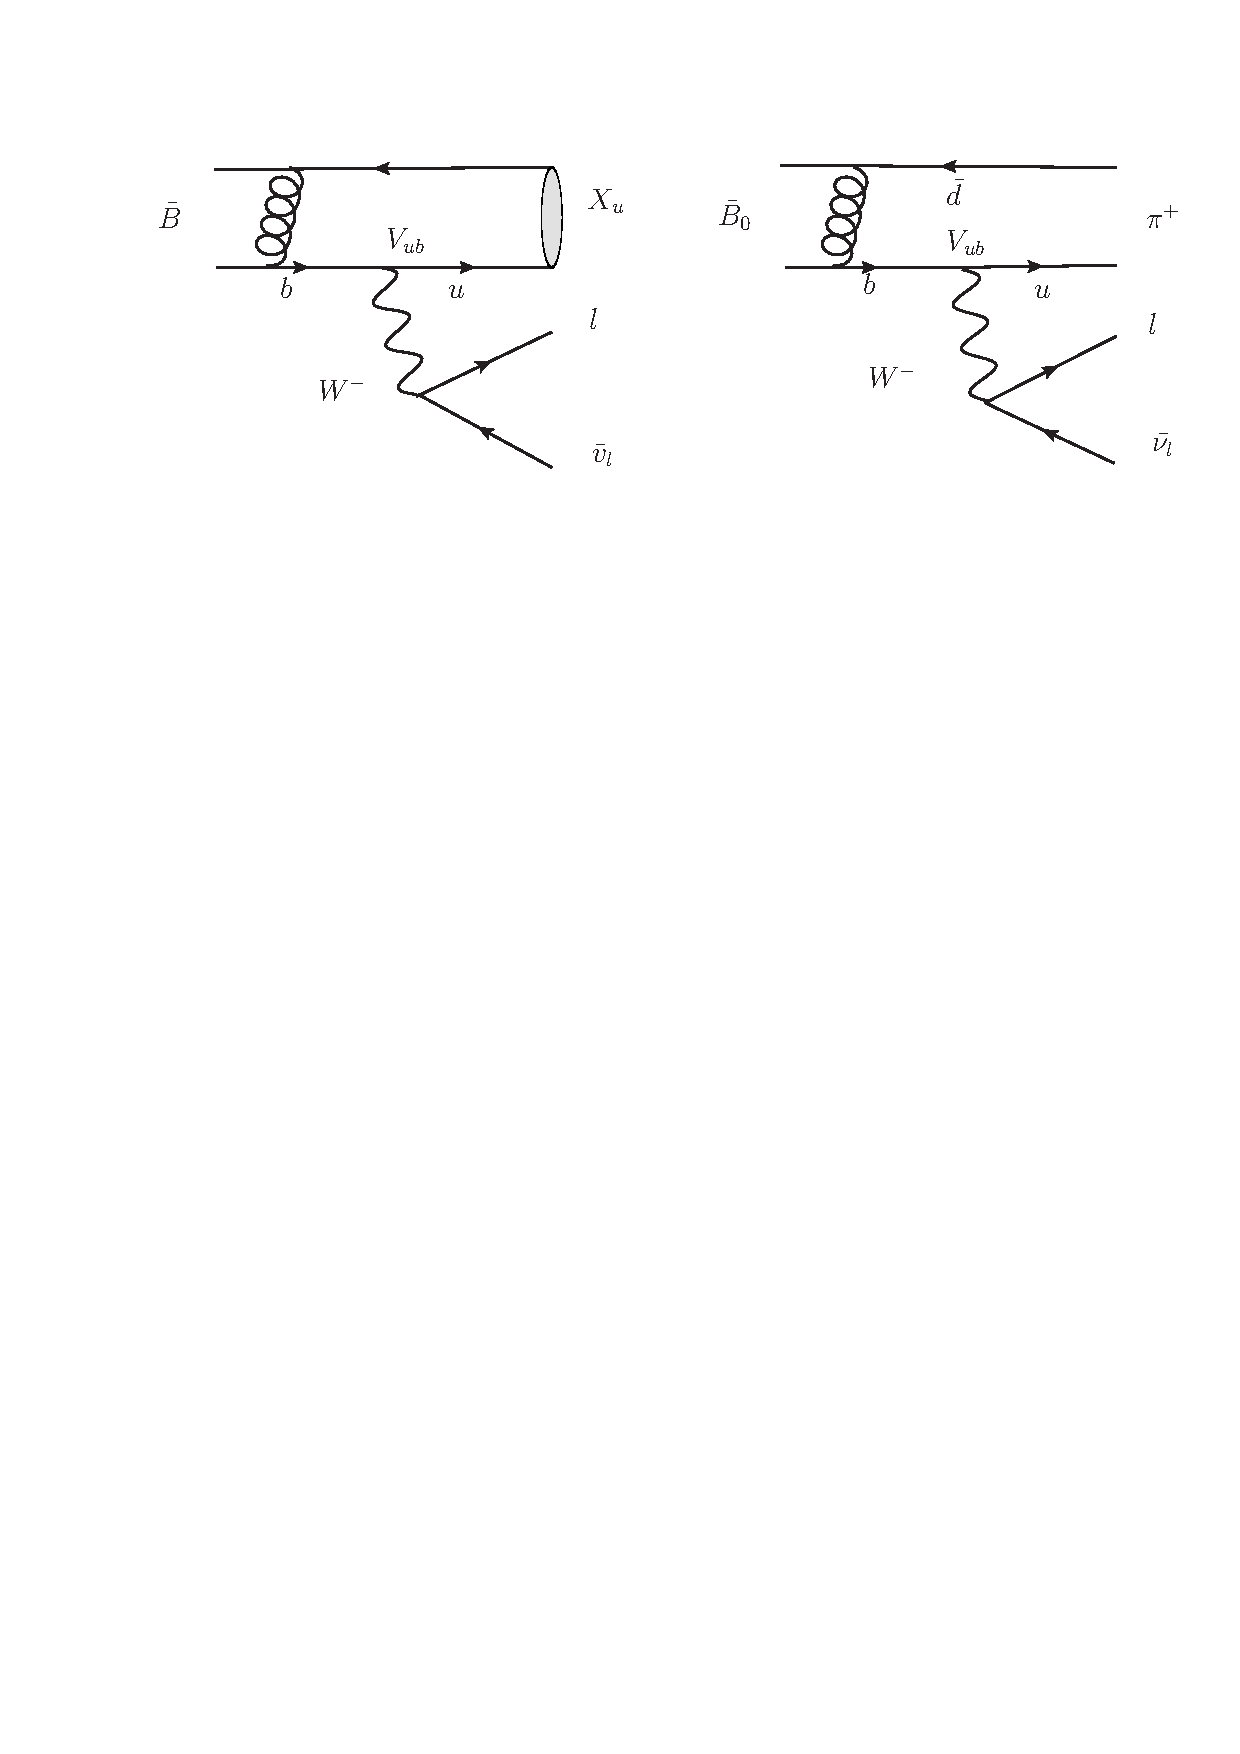
\includegraphics[trim = 15mm 215mm 0mm 25mm, clip, width=8cm]{incl_ex_feyn.pdf} 
        \end{center}
        \hspace{1.cm} \footnotesize{$|V_{ub}| = (4.41 \pm 0.15 ^{+ 0.15} _{-0.17}) \times 10^{-3}$} \hspace{0.3cm} \footnotesize{$|V_{ub}| = (3.23 \pm 0.31) \times 10^{-3}$}
  
  \vspace{0.1cm}
       \begin{itemize}
  \item \normalsize{Leptonic B decays ($B^{+} \rightarrow \tau^{+} \nu_{\tau}$):}
      \begin{center}
       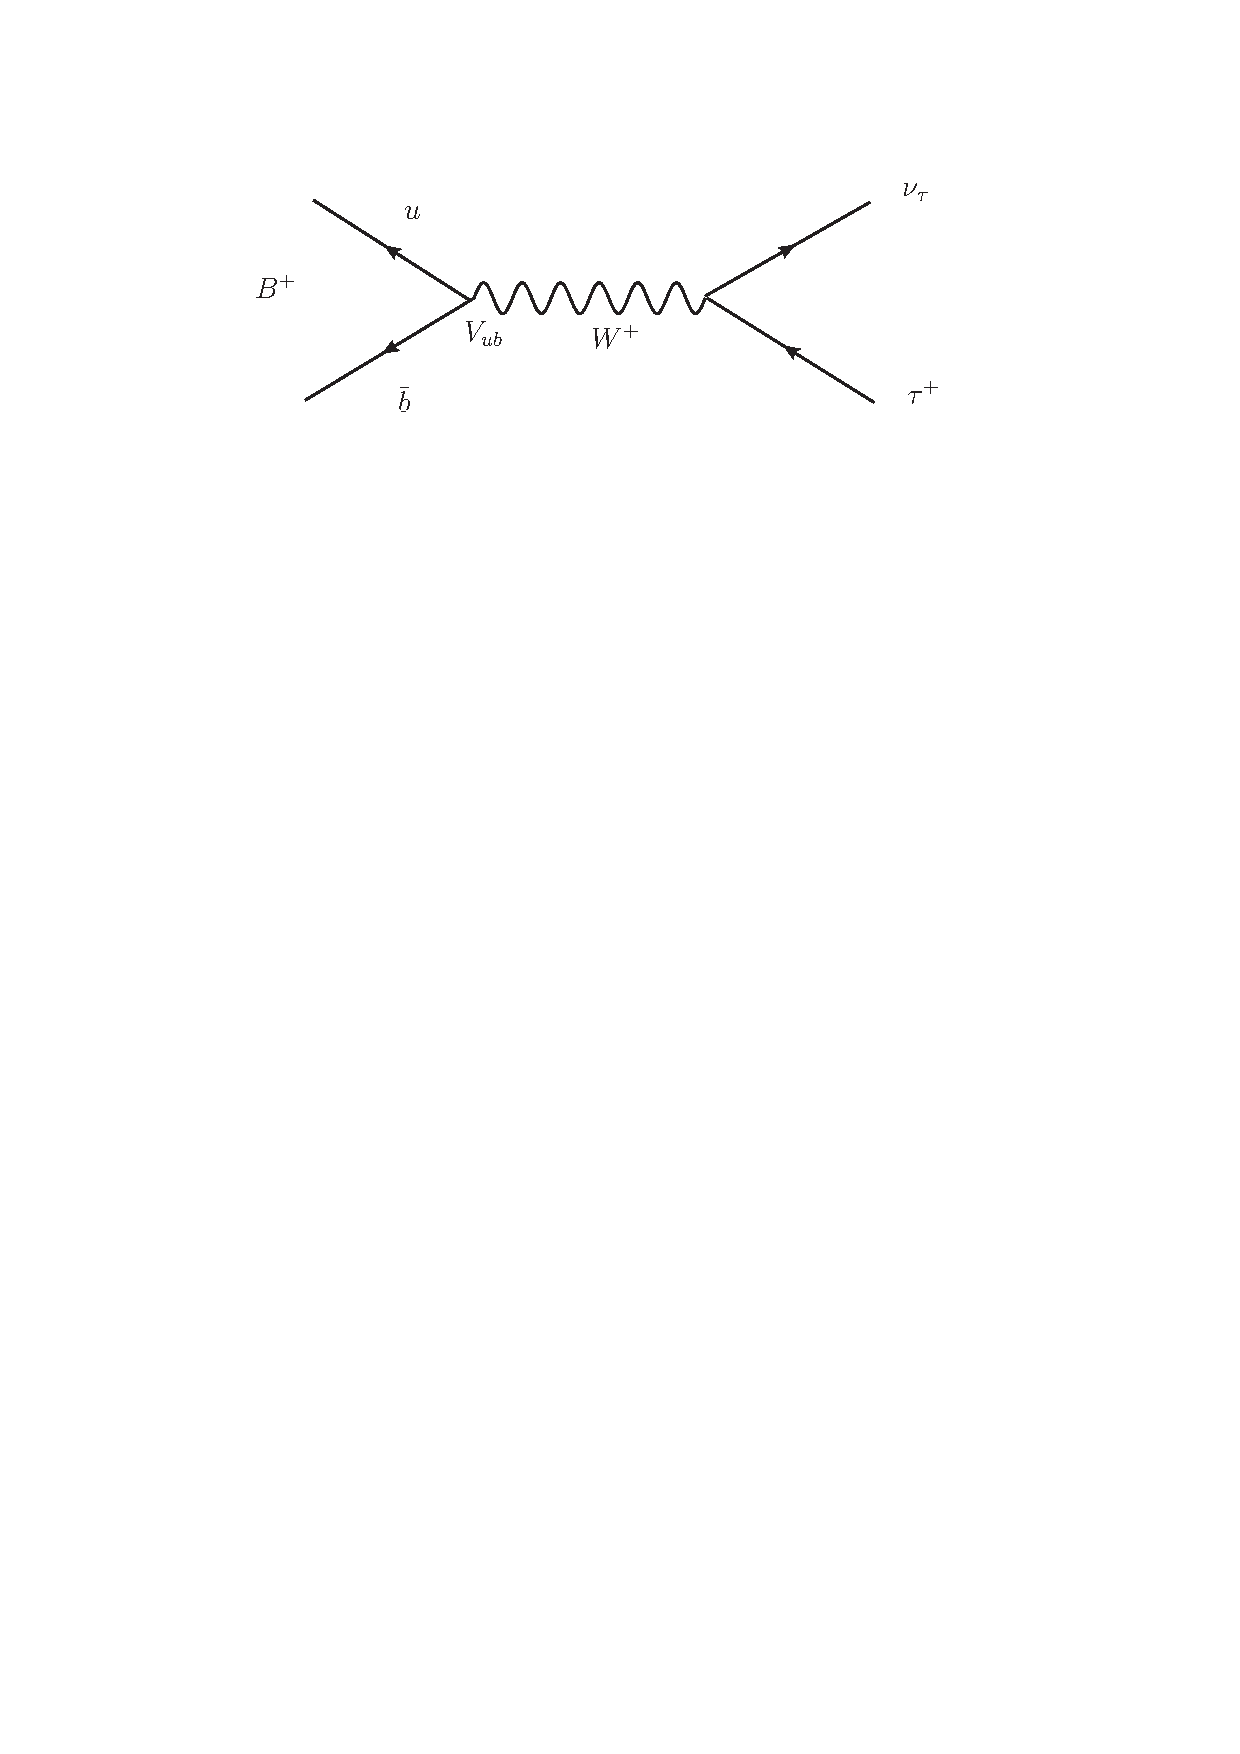
\includegraphics[trim = 15mm 215mm 0mm 30mm, clip, width=8cm]{lepfeyn.pdf} 
       \end{center}
   \end{itemize}
  

}







 \frame{
 \frametitle{Exclusive Measurements of $|V_{ub}|$} 


            \begin{columns}[T]
   \begin{column}{.5\textwidth}
   \begin{center}
\begin{itemize}
  \setlength{\itemsep}{12pt}
\item BaBar, Belle and CLEO: \\
$|V_{ub}| = (3.23 \pm 0.31) \times 10^{-3}$
  \item Exclusive Approach:
   \begin{itemize}
     \setlength{\itemsep}{5pt}
  \item Exclusive final state ($\bar{B}_{0} \rightarrow \pi^{+} \l^{-} \bar{\nu}_{l}$)
  \item $\frac{d \Gamma}{d q^{2}} = \frac{G_{F}^{2} |V_{ub}|^{2}}{24 \pi^{3}} |p_{\pi}|^{3} | f_{+} (q^{2})|^{2}$ 
  \item $ | f_{+} (q^{2})|^{2}$ predicted by lattice QCD
  \item Uncertainty dominated by $ | f_{+} (q^{2})|^{2}$.
  \end{itemize}
  \end{itemize}
  \end{center}
  \end{column}
      \begin{column}{.5\textwidth}
      % \footfullcite{gfgfg}

      
  \begin{center}
   \footnotesize{ \uline {Measured partial branching fraction  \\ $\Delta B (\bar{B}_{0} \rightarrow \pi^{+} \l^{-} \bar{\nu}_{l})$ [2]}:}
   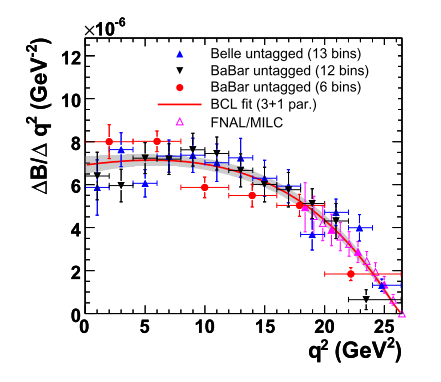
\includegraphics[width=1.0\textwidth]{BF2.png} 
\end{center}
    \end{column}
  \end{columns}

  \vspace{0.8cm}
   \tiny{[2] J. Beringer et al., Determination of $V_{ub}$ and $V_{cb}$ (Particle Data Group). \textit{Phys. Rev.} D\textbf{86}, 010001 (2012).}
}





 

 \frame{
 \frametitle{ Current $B_{s} \rightarrow K \mu \nu$ Stripping Selection }


  
  \begin{tabular}{l*{9}{c}r}
Kaon cuts& Muon cuts & Mother cuts   \\
\hline
$P > 3000$ MeV/c & $P > 3000$ MeV/c & \textcolor{red}{$cos \theta_{B_{s}Y} > 0.99$}  \\
$p_{\text{T}} > 800 MeV/c $        &$p_{\text{T}} > 800 MeV/c$ & $\textcolor{red}{E_{\nu} < 2000} $ \textcolor{red}{MeV}     \\
Track $\chi^{2} <  6.0 $        & Track $\chi^{2} <  4.0 $ & Vertex $\chi^{2} < 2.0$  \\ 
Min IP $\chi^{2} > 16.0$ & Min IP $\chi^{2} > 12.0$ &  $\chi^{2}$ sep. from PV $> 100.0$\\
$\Delta LL(K-p) > 0$ & $\Delta LL(\mu-p) > 0$&  \\
$\Delta LL(K-\pi) > 5 $ & $\Delta LL(\mu-\pi) > 3$& \\
$\Delta LL(K-\mu) > 0 $ & $\Delta LL(\mu-K) > 0$&
\end{tabular}

\begin{itemize}
 \setlength{\itemsep}{5pt}
\item StdLooseMuons and StdLooseKaons selections also used.
\item Track Ghost probability $< 0.5$
\item Combination cut: $\textcolor{red}{1500 MeV/c^{2} \leq M_{K\mu} \leq 5500 MeV/c^{2}}$.
\end{itemize}

}

\frame{
 \frametitle{RICH PID performance}

  \begin{center}
 
    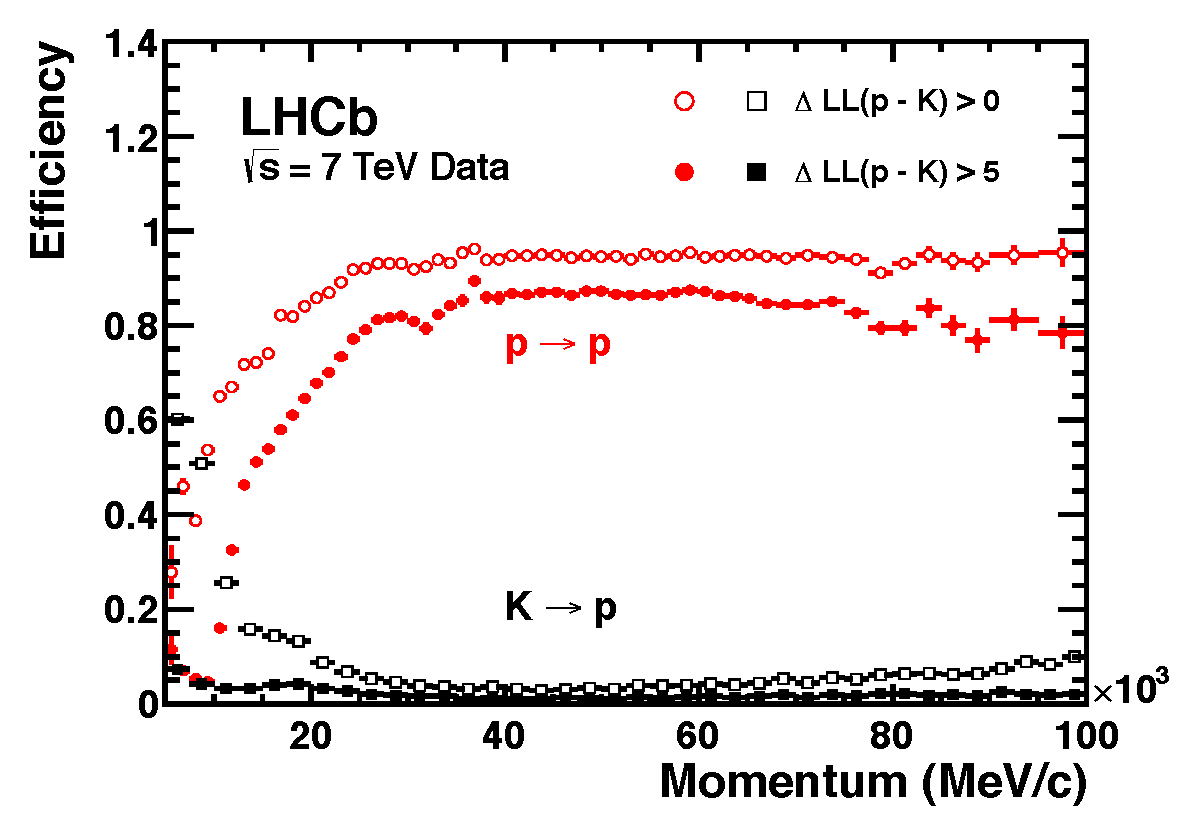
\includegraphics[width=0.5\textwidth]{pk.pdf}  
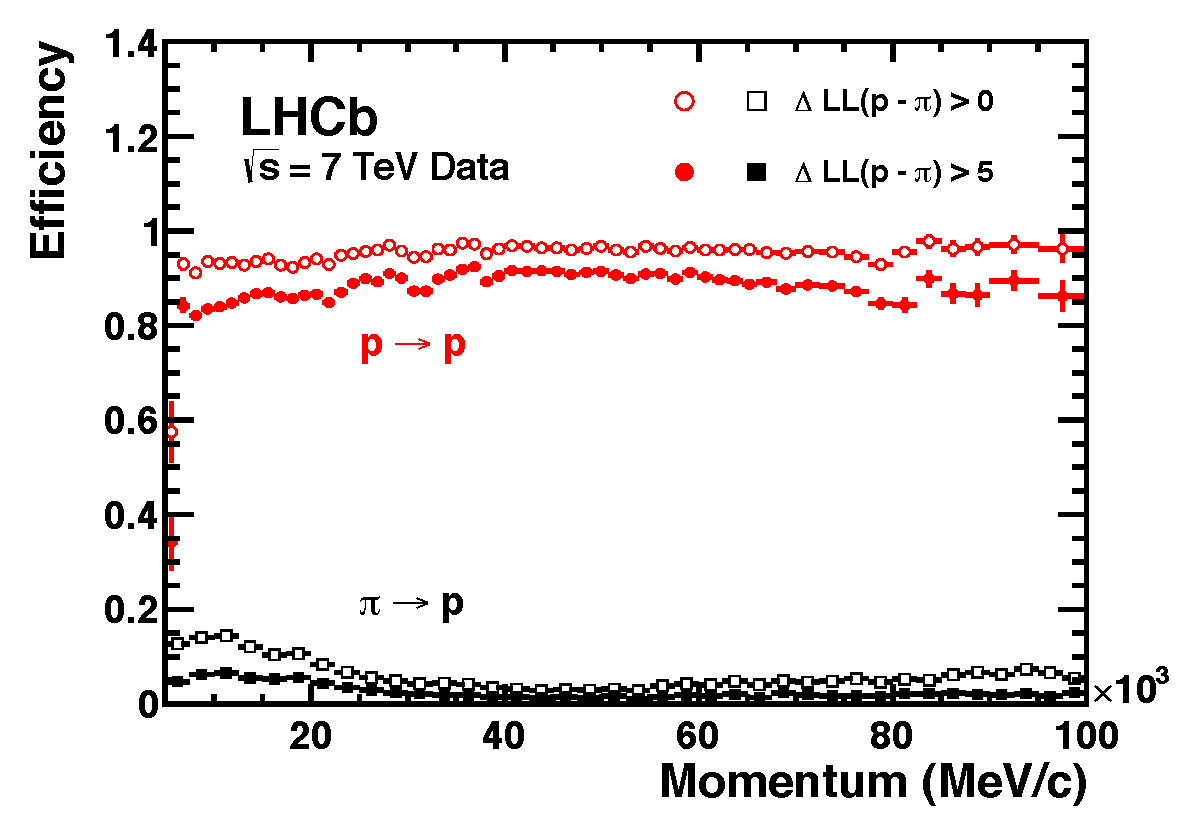
\includegraphics[width=0.5\textwidth]{pionp.pdf} 
\begin{itemize}

  \item High $K$-$p$ misidentification rate / low $p$-$p$ identification efficiency below $15$ GeV/c.
\end{itemize}
\end{center}

}

}

 \frame{
 \frametitle{ Stripping Efficiency for Signal }
 
 \begin{itemize}
  \setlength{\itemsep}{5pt}
    \item No available $\Lambda_{b} \rightarrow p \mu \nu$ MC sample yet.
    \item Strip $B_{s} \rightarrow K \mu \nu$ 2011 MC sample using existing line +  $P_{K} > 10$ GeV/c.
    \item Signal Efficiency for stripping:   $ 7.2 \pm 0.1 \%$.
     \item Acceptance, $ A \approx 1.4\%$.
     \item In $1$ fb$^{-1}$ expect: \\ $N_{Events} = 2 \times \sigma(b\bar{b}) \times f_{\Lambda_{b}} \times \Lagr  \times B(\Lambda_{b} \rightarrow p \mu^{-} \bar{\nu}) \times A$ \\
    \vspace{0.3cm} Taking $ f_{\Lambda_{b}} \sim 0.25$, $ B(\Lambda_{b} \rightarrow p \mu^{-} \bar{\nu}) \sim 10^{-4}$, $\sigma(b\bar{b}) \sim 280 \mu$b \\
    \vspace{0.3cm} $N_{Events} \approx  2 \times 10^{5}$

\end{itemize}
}


 
  \frame{
 \frametitle{ $B_{s} \rightarrow K \mu \nu$ MC $q^{2}$ distribution  }
 \begin{itemize}
  \setlength{\itemsep}{5pt}
   \item Remove certain cuts to investigate their impact.
    \item $E_{\nu}$ cut kills the endpoint of the $q^{2}$ distribution.
   \end{itemize}
  \begin{center}
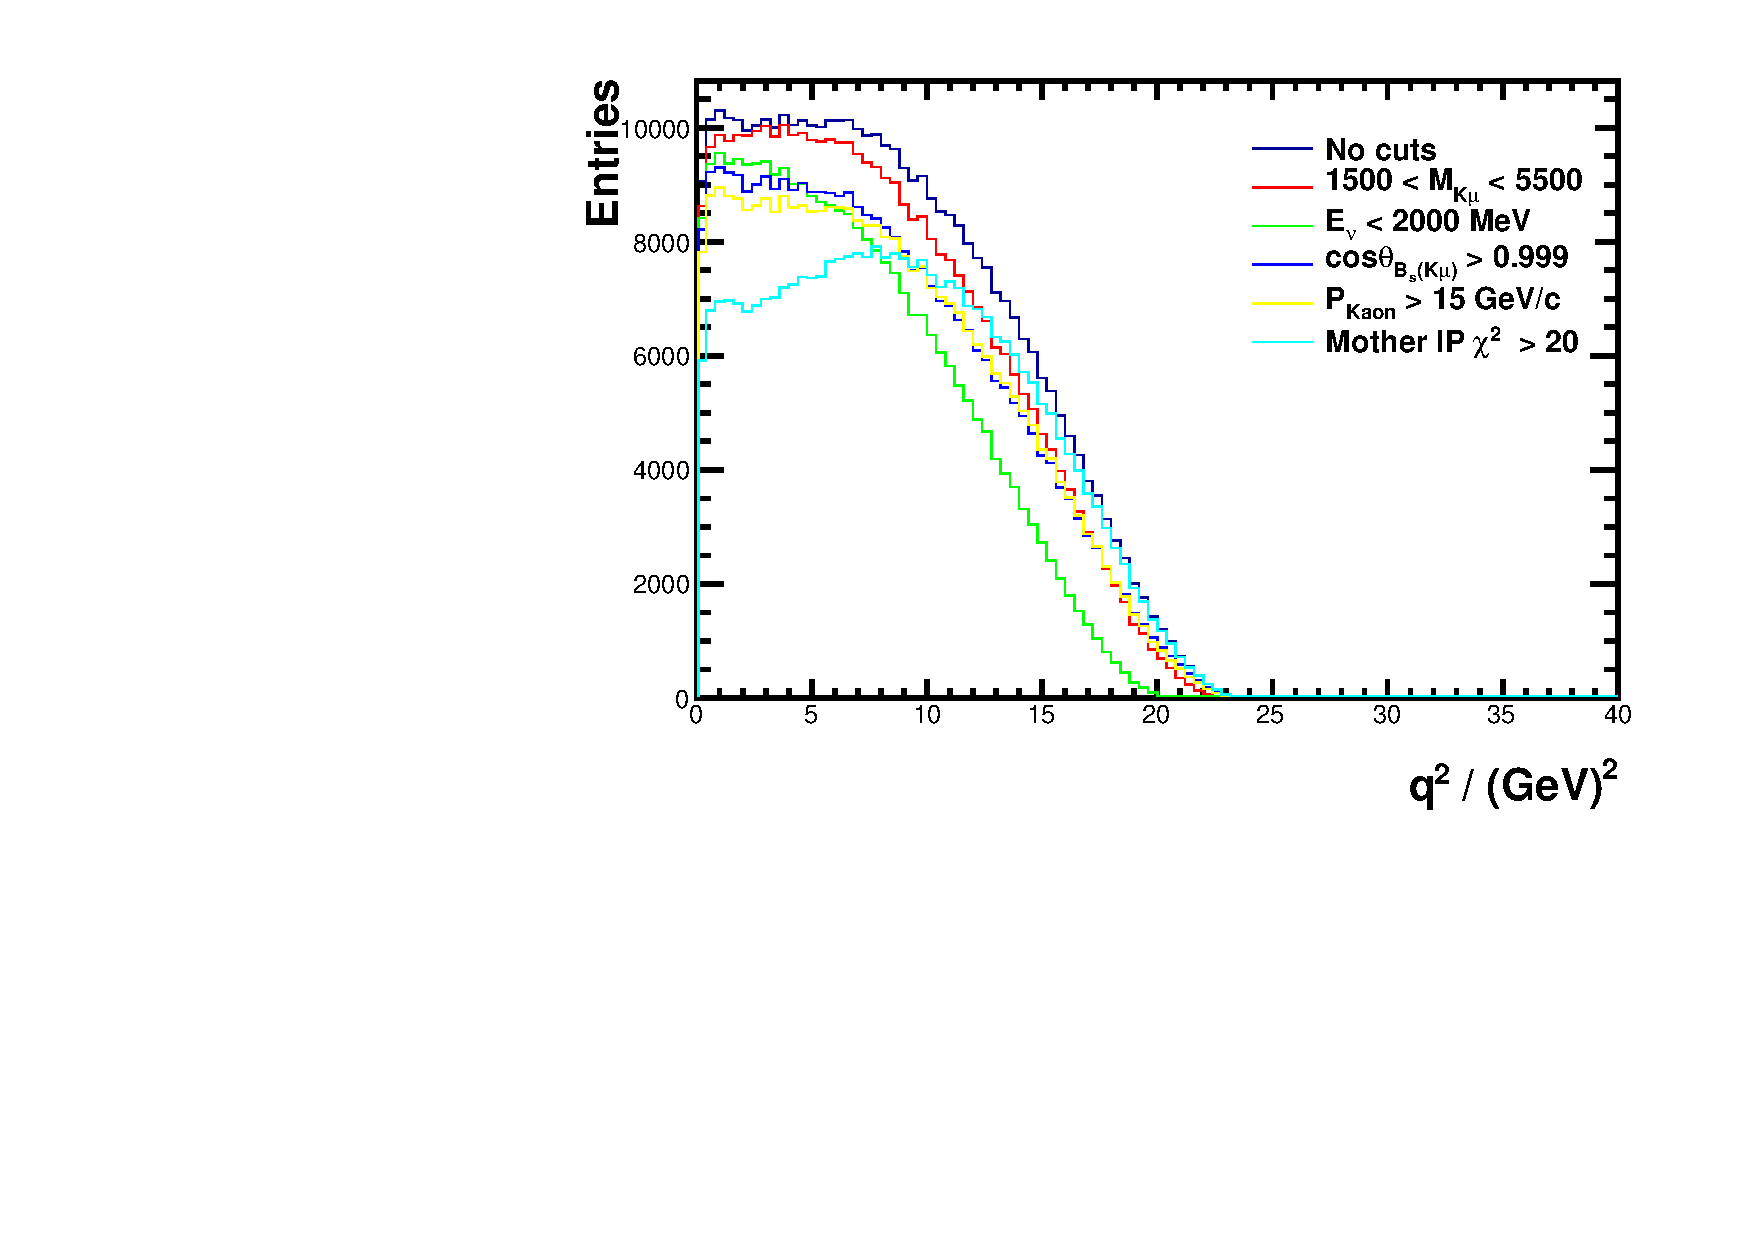
\includegraphics[width=8cm]{Bs_Kmunnu_MC_qsquared.pdf} 
\end{center}
}

 \frame{
 \frametitle{ $\Lambda_{b} \rightarrow p \mu \nu$ Line }
 
 \begin{itemize}
    \item $\Lambda_{b} \rightarrow p \mu \nu$ stripping line based on the current $B_{s} \rightarrow K \mu \nu$ line.
    \item Remove $E_{\nu}$ cut.  Demand $P_{proton} > 15$ GeV/c and $1000$ MeV/c$^{2} \leq M_{p\mu} \leq 5600$ MeV/c$^{2}$.  
    \item Test using TestMyStrippingLineOn2012Data\_Reco14.py script (100,000 events):
\end{itemize}

\begin{tabular}{l*{4}{c}r}
$L_{b}\rightarrow p \mu \nu$ line             & Retention (\%) & Accepted & ms/evt  \\
\hline
Above cuts & 0.449 & 449 & 0.474   \\
$2000$ MeV/c$^{2} \leq M_{p\mu}$  & 0.246 & 246 & 0.386  
\end{tabular}

 \begin{itemize}
    \item Require retention $< 0.05 \%$ and timing $< 0.5$ ms/evt.
\end{itemize}
}

  \frame{
 \frametitle{}
\hspace{1.5cm}  \uline{$M_{p\mu}$ and $E_{\nu}$ Distributions using 2012 test data}
  \begin{center}
 
    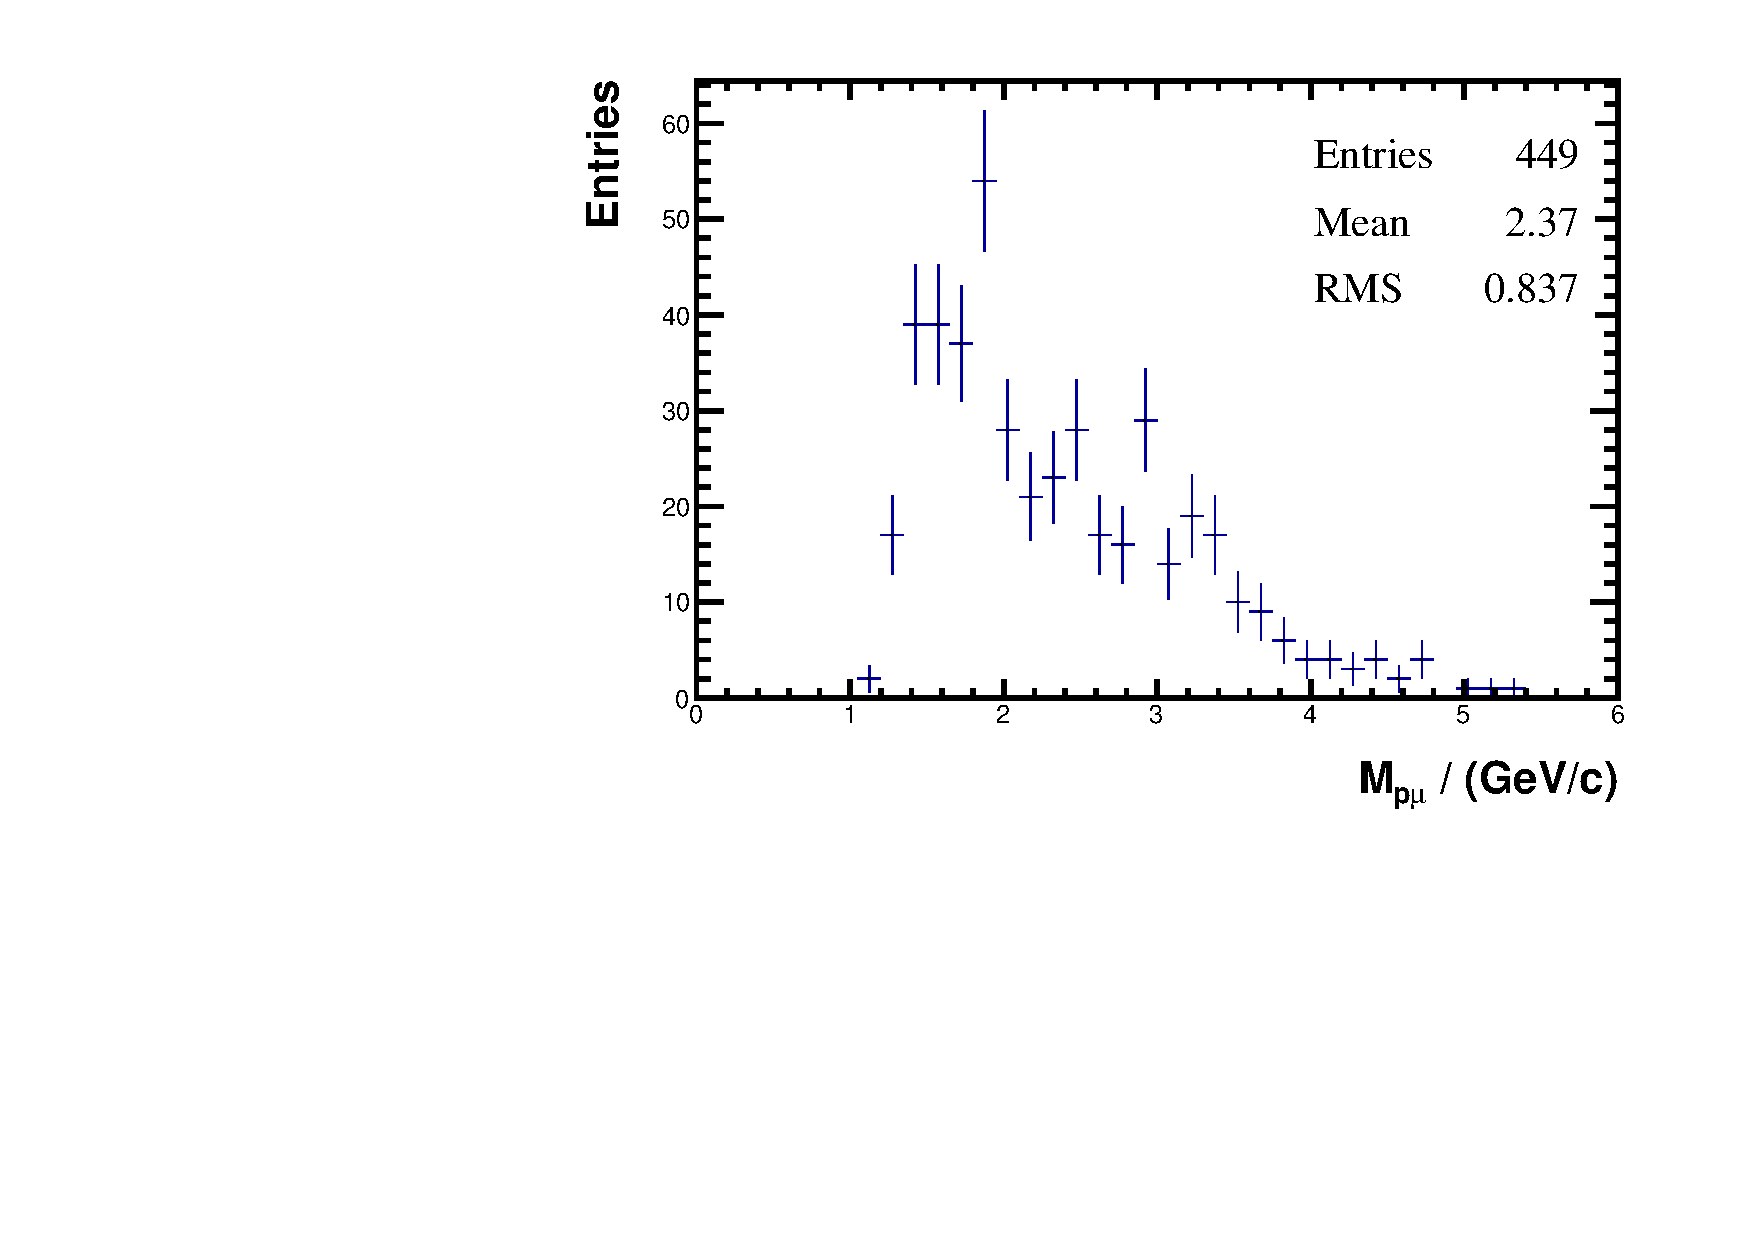
\includegraphics[width=0.4\textwidth]{Mpmu.pdf}  
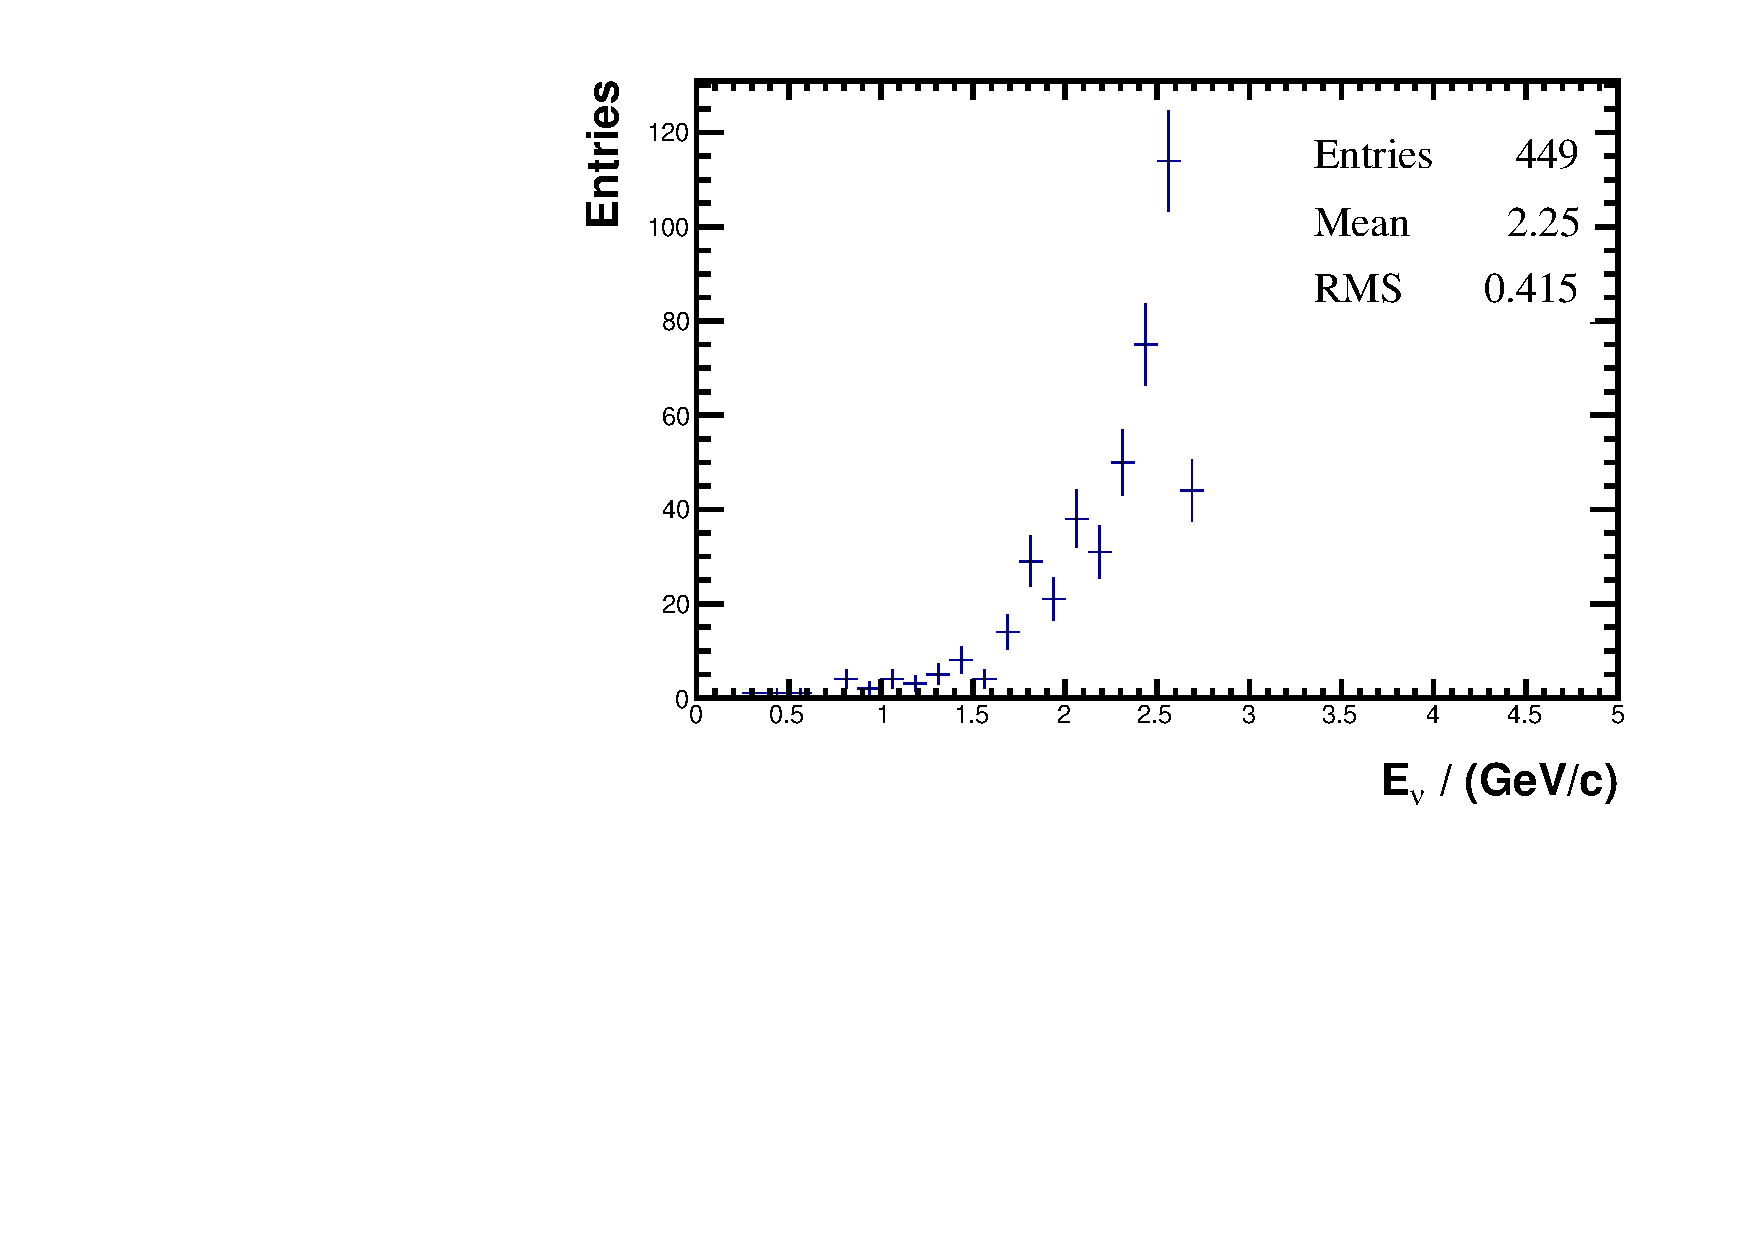
\includegraphics[width=0.4\textwidth]{Enu.pdf} 

\end{center}
\hspace{1cm}  \uline{$M_{p\mu}$ and $E_{\nu}$ Distributions for generator level $\Lambda_{b} \rightarrow p \mu \nu$}
  \begin{center}
 
    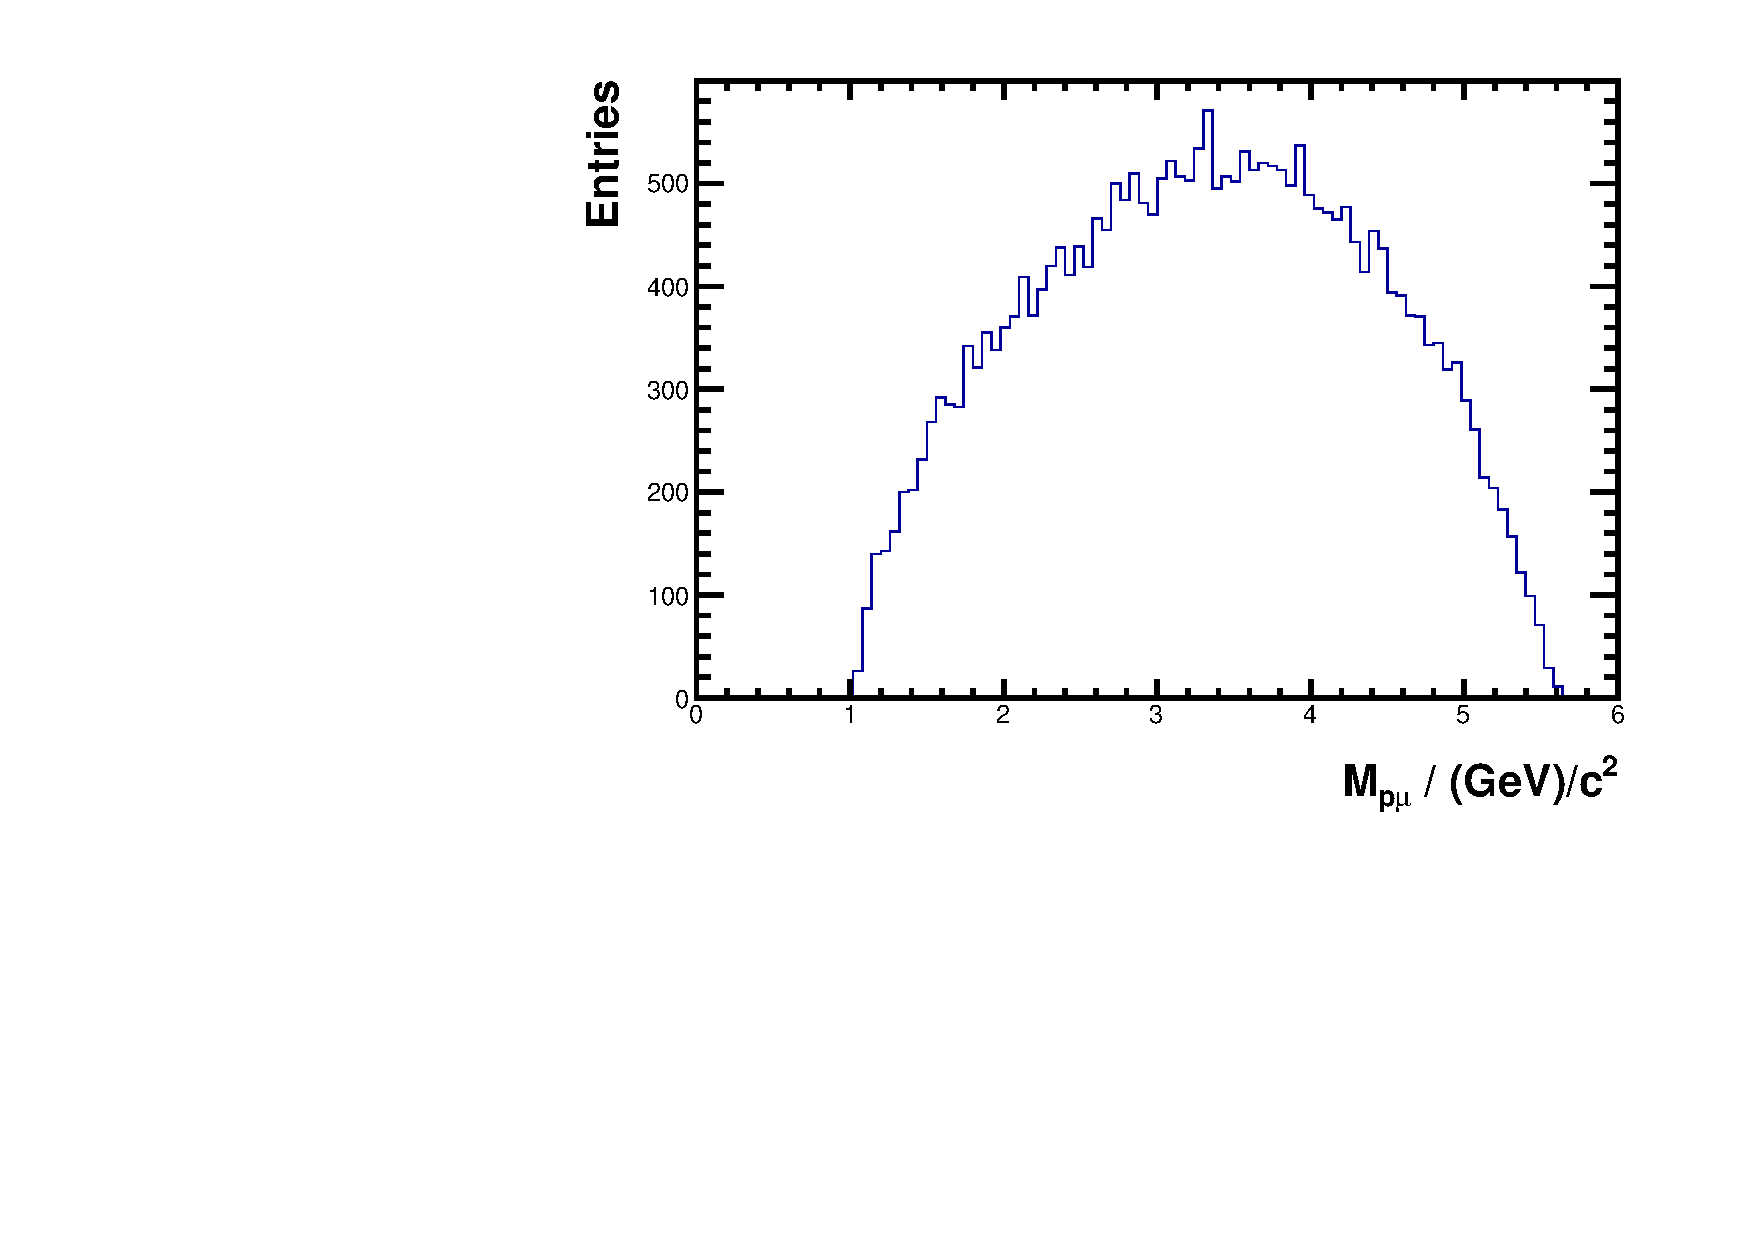
\includegraphics[width=0.4\textwidth]{signal_Mpmu.pdf}  
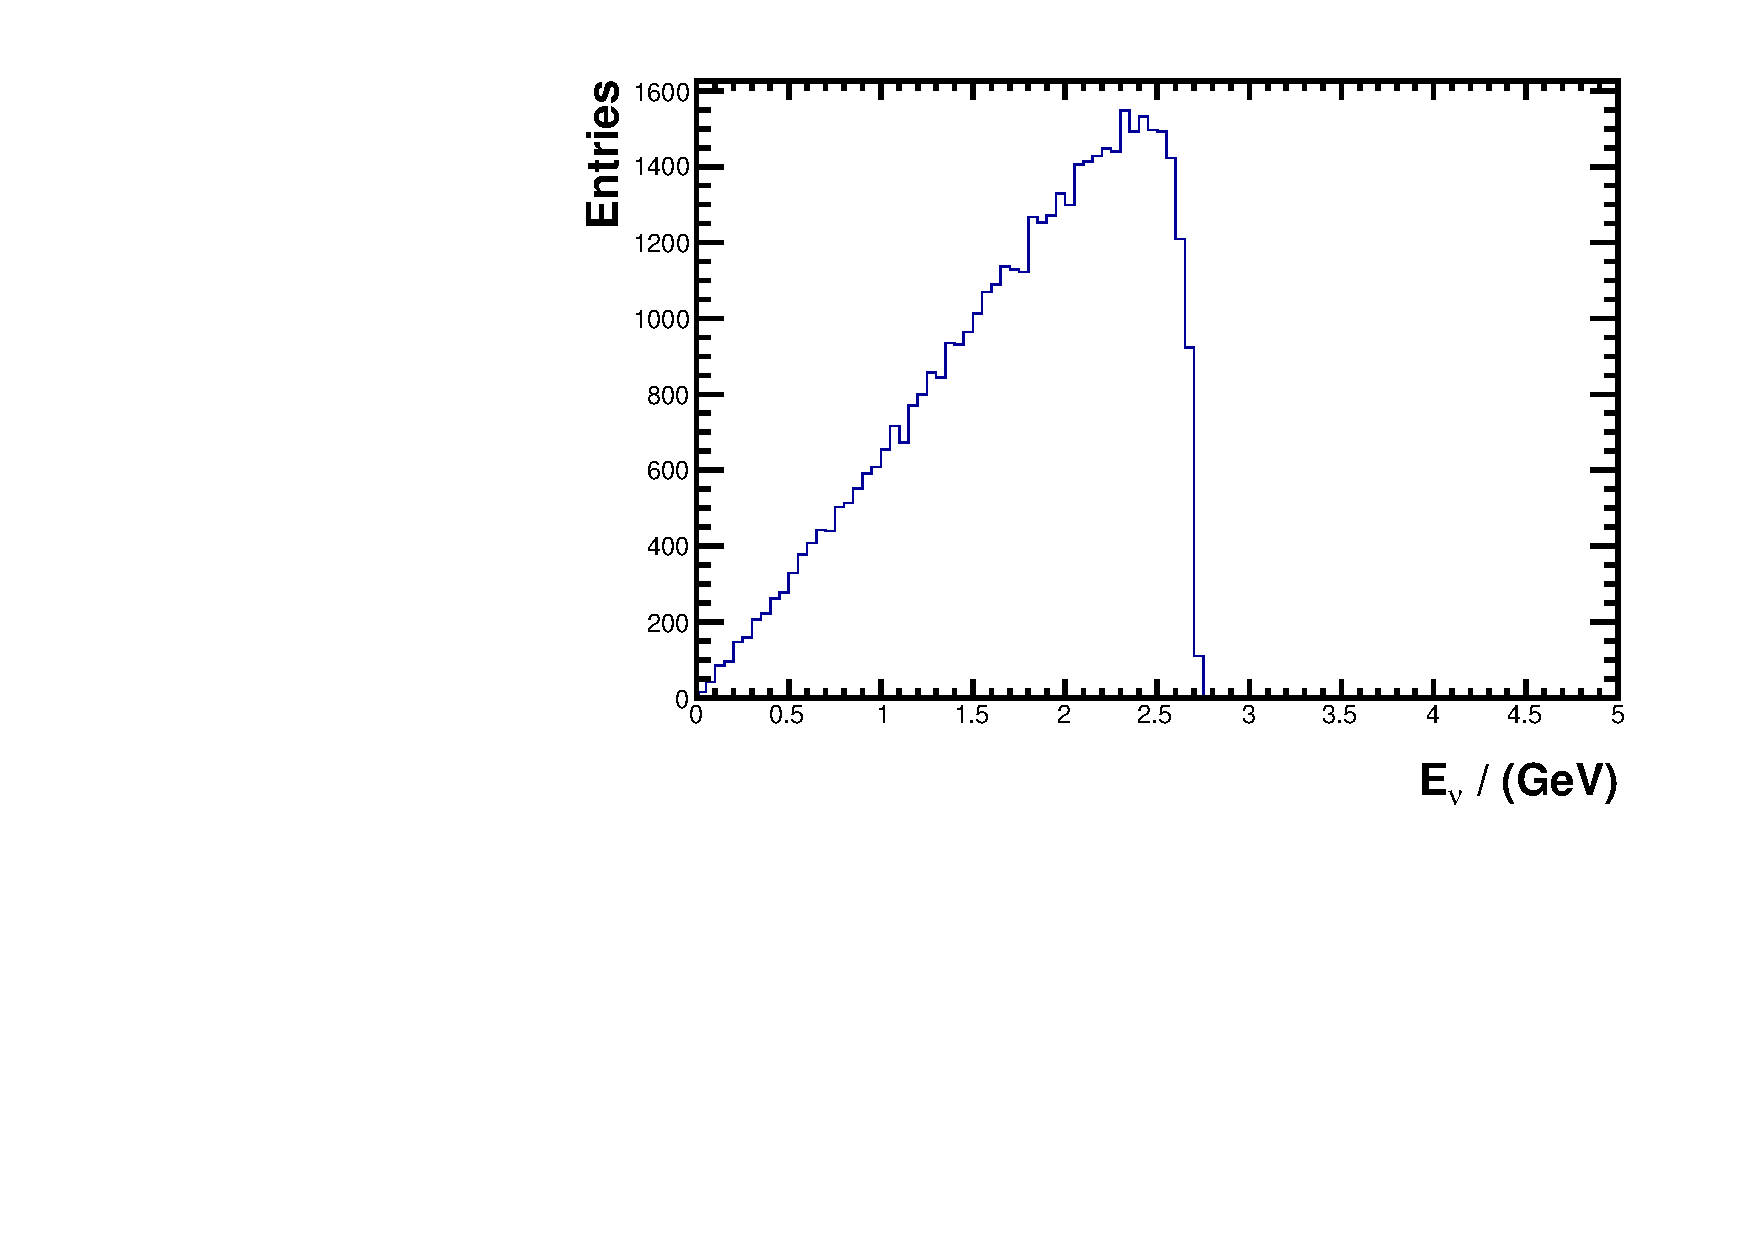
\includegraphics[width=0.4\textwidth]{Enu_signal.pdf} 

\end{center}

}

  \frame{
 \frametitle{}
 
 \hspace{1cm}  \uline{$\Lambda_{b} \rightarrow p \mu \nu$ generator level $q^{2}$ distribution}

  \begin{center}
 
    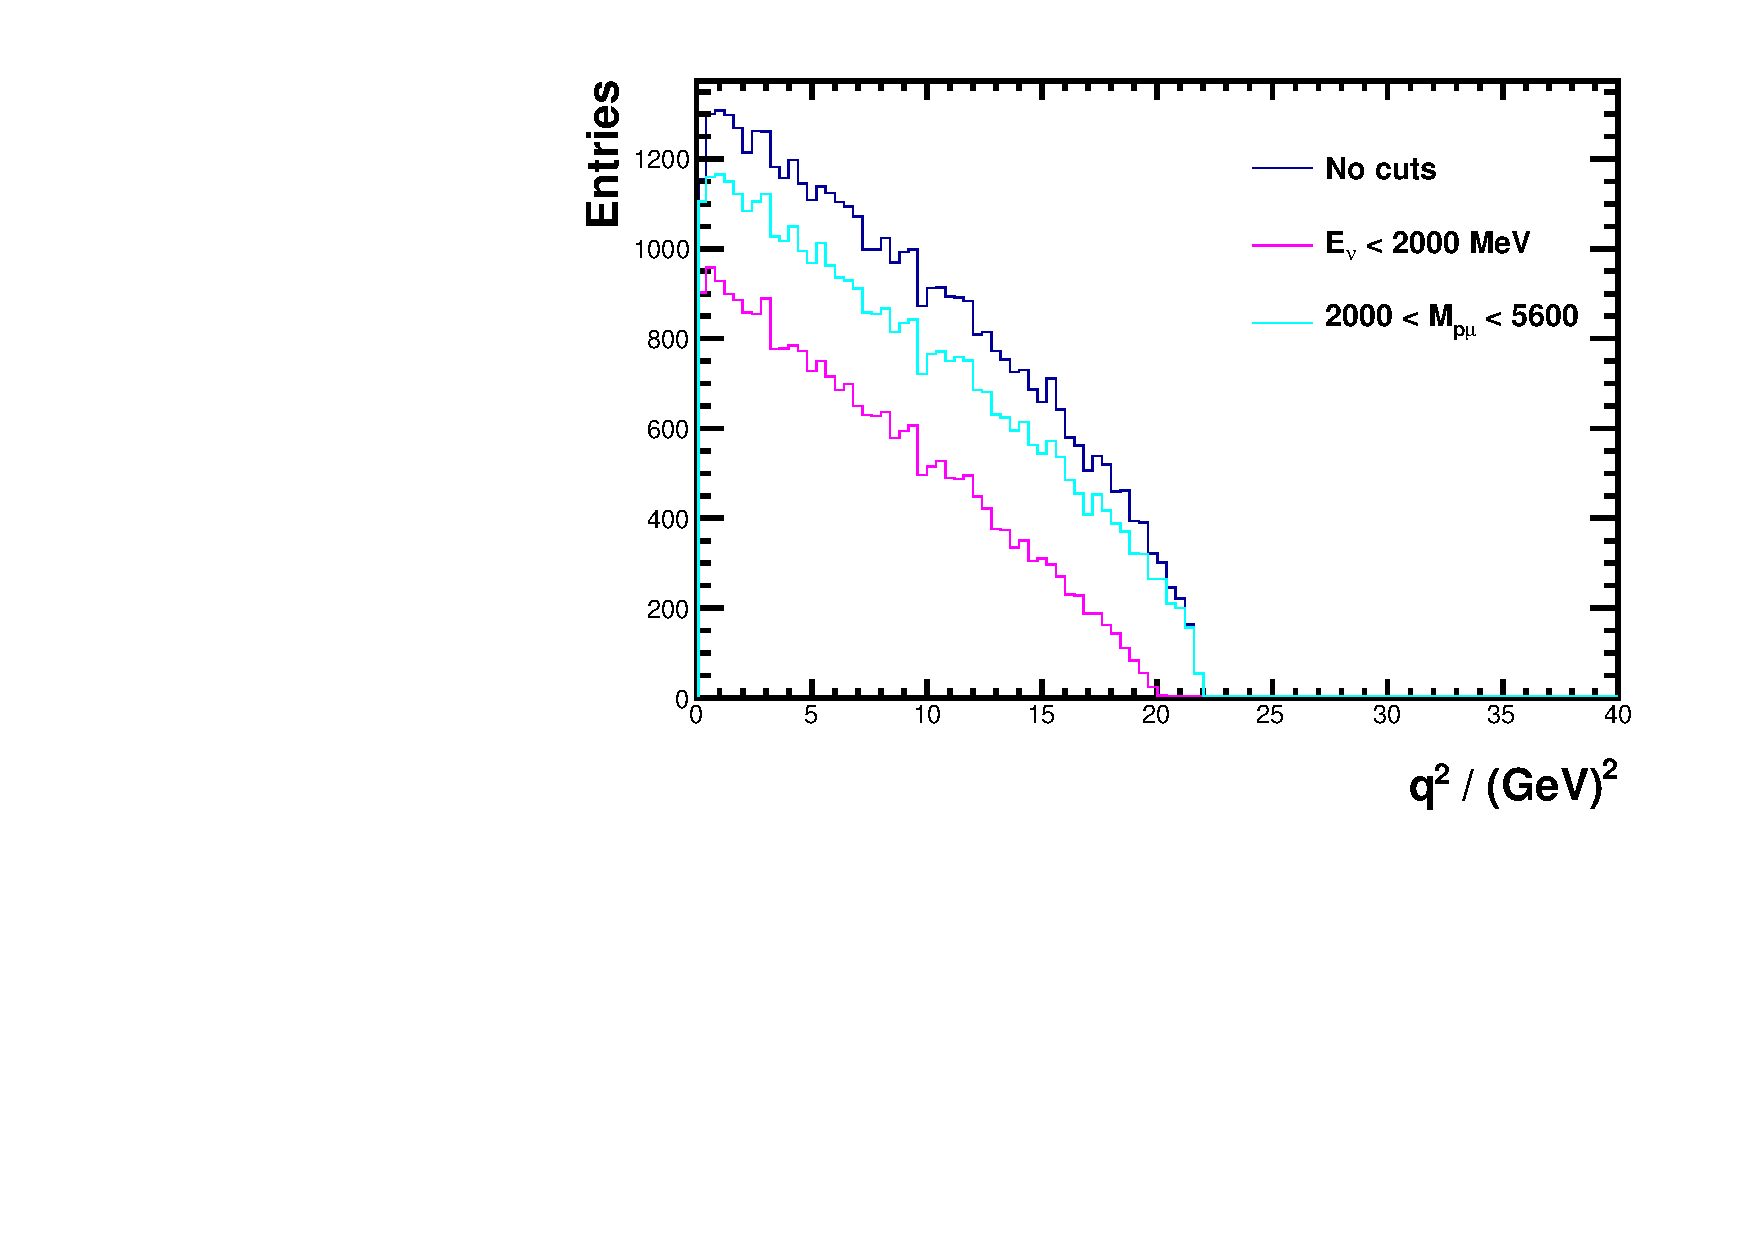
\includegraphics[width=0.8\textwidth]{qsquared.pdf}  
\end{center}


}

  \frame{
 \frametitle{Conclusion}
 \begin{itemize}
  \setlength{\itemsep}{5pt}
   \item $E_{\nu}$ cut kills the $q^{2}$ endpoint.
    \item Additional cuts required to reduce retention to $<0.05\%$.
    \item $\Lambda_{b} \rightarrow p \mu \nu$ MC approved (1 million events).
    \item Presenting to the Semi-leptonic working group tomorrow.
   \end{itemize}

}


 \end{document}